\documentclass[11pt,letterpaper]{article}
\usepackage{fullpage}
\usepackage[top=2cm, bottom=4.5cm, left=2.5cm, right=2.5cm]{geometry}
\usepackage{amsmath,amsfonts,amssymb}
\usepackage{lastpage}
\usepackage[inline]{enumitem}
\usepackage{fancyhdr}
\usepackage{mathrsfs}
\usepackage{xcolor}
\usepackage{graphicx}
\usepackage{hyperref}
\hypersetup{colorlinks=true, linkcolor=blue, linkbordercolor={0 0 1}}

\renewcommand{\arraystretch}{1.75}

\setlength{\parindent}{0.0in}
\setlength{\parskip}{0.05in}

\pagestyle{fancyplain}
\lhead{Brad Cownden}
\chead{}
\rhead{April 30, 2020}
\cfoot{\small\thepage}
\headsep 36pt

\begin{document}
\vspace{.2in}
\begin{center}
    {\bf GPU Solutions for PSCAD: IT17112}
\end{center}

	\vspace{.25in}

\begin{tabular}{| p{0.2\textwidth} | p{0.75\textwidth} |}
	\hline
	Reporting Period & April 23, 2020 - April 30, 2020 \\ \hline

	Activities & \begin{enumerate*}
	\item[\tiny\textbullet] Discussed discrepancies in the results from CPU and GPU methods with MHI, in particular the issues at lines 2208-2210. \newline
  \item[\tiny\textbullet] Plotted relative difference between CPU and GPU results for a specific time step (see figure~\ref{fig: rel diff}). \newline
  \item[\tiny\textbullet] Issues with these entries are known to MHI and are due to the \emph{Province} sample case being ill conditioned. \newline
  \item[\tiny\textbullet] Continued to develop solution for running NSight Eclipse in a container on the U of W servers. X11 forwarding through ssh tunnel remains an issue. \newline
	\end{enumerate*} \\ \hline

	Issues & \begin{enumerate*}
	\item[\tiny\textbullet] X11 forwarding from within a container needs to be resolved or a new strategy developed.
	\end{enumerate*} \\ \hline

	Milestones \newline Accomplished & \begin{enumerate*}
	\item[\tiny\textbullet] Resolved the observed jump in relative differences between GPU and CPU solving methods.
  \end{enumerate*} \\ \hline

	Milestones Not \newline Accomplished & \begin{enumerate*}
	\item[\tiny\textbullet] Run QRFactor on U of W servers
	\end{enumerate*} \\ \hline

	Next Week's \newline Milestones & \begin{enumerate*}
	\item[\tiny\textbullet] Compare QRFactor results from CPU and GPU methods for standardized sparse data sets, and for unit vectors. \newline
  \item[\tiny\textbullet] Compare NVIDIA solutions (both CPU and GPU) with solutions from tested methods, such as Eigen.
	\end{enumerate*} \\ \hline

	Forwarded Issues & \begin{enumerate*}
	\item[\tiny\textbullet] \item[\tiny\textbullet] Resolve X11 forwarding from within container in order to run NSight Eclipse through Docker
	\end{enumerate*} \\ \hline
\end{tabular}

\begin{figure}[h]
  \centering
  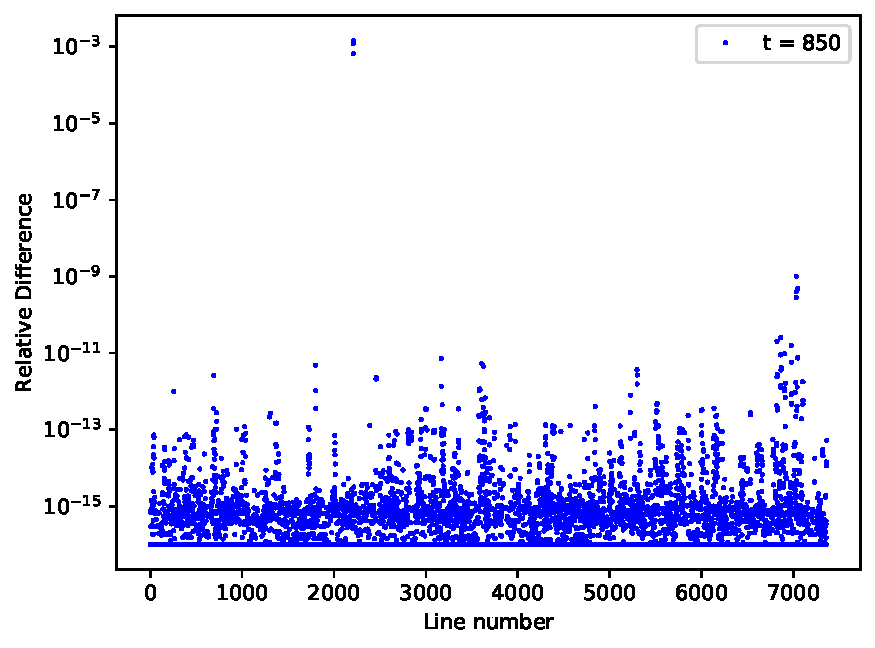
\includegraphics[width=\textwidth]{C:/Users/bradc/Documents/MHI/QRFactor/CPUvsGPUFactor2}
  \caption{Relative difference between CPU and GPU solving methods as a function of line number for time step $t = 840$. A lower bound of $10^{-16}$ was used for comparison purposes. Note that values of the three previously identified lines, 2208-2210, are several orders of magnitude larger than the next nearest values.}
  \label{fig: rel diff}
\end{figure}

\end{document}
